\chapter{Definizione del percorso di stage}
\label{chap:Definizione-del-percorso-di-stage}

\section{Il rapporto tra azienda e \textit{stage}}
Come già accennato nella sotto-sezione \ref{Propensione-all'-innovazione}, VisioneImpresa investe molte risorse nei progetti di \textit{stage}, ritenendo che questi siano uno strumento concreto ed efficace per promuovere l'innovazione e la sperimentazione.
Durante il mio periodo di tirocinio erano presenti, oltre a me, altri quattro \textit{stagisti}. Quasi tutti erano impegnati in progetti differenti e ritenuti rilevanti dall'azienda. Questo dato testimonia quanto VisioneImpresa ritenga importante questo tipo di rapporto con gli studenti e gli enti del territorio. In quanto società \textit{benefit} l'azienda persegue anche obiettivi sociali, tra i quali la collaborazione con scuole e università attraverso progetti orientati all'innovazione.
Gli \textit{stagisti} provengono principalmente da corsi di laurea triennali in informatica o ingegneria informatica, portando con loro le conoscenze accademiche acquisite negli anni. Lo \textit{stage} ha una durata di 300-320 ore un tempo che consente allo studente di contribuire in maniera concreta allo sviluppo di soluzioni aziendali, e allo stesso tempo conferisce un esperienza significativa dal punto di vista professionale.
I progetti presentati dall'azienda non hanno un obiettivo prettamente formativo, ma corrispondono a necessità reali dell'azienda, emerse tramite il confronto con clienti o con \textit{team} di sviluppo interni. I tirocinanti si trovano quindi immersi nel contesto aziendale con l'obiettivo di affrontare problematiche concrete, analizzare e riscrivere codice esistente e approfondire tecnologie, situazioni spesso nuove per uno studente.
Alla fine del periodo ciascun tirocinante presenta il lavoro svolto al \textit{team} di sviluppo più appropriato e al referente aziendale, questa fase è cruciale per rendere possibile la valutazione del lavoro svolto e spiegare il progetto da un punto di vista tecnico ponendo le basi per una possibile futura integrazione di esso nei prodotti aziendali.
Inoltre VisioneImpresa utilizza il periodo di \textit{stage} anche come momento per valutare il profilo dello studente, sia a livello tecnico che a livello personale. In diversi casi, il tirocinio si è trasformato in un'opportunità concreta di inserimento nel contesto lavorativo, rendendo possibile agli studenti di proseguire il percorso all'interno dell'azienda.



\section{Proposte progettuali dell'azienda}
Il primo contatto con VisioneImpresa è avvenuto grazie l'evento StageIT 2025, organizzato dall'università di Padova per mettere in contatto studenti alla ricerca di un tirocinio e aziende del territorio che propongono offerte di \textit{stage} in ambito informatico. 
Durante l'evento ho avuto modo di svolgere numerosi colloqui con aziende interessanti, che proponevano una vasta scelta di progetti distribuiti su molti ambiti applicativi.
Nonostante durante l'evento no abbia svolto un colloquio diretto con VisioneImpresa, sono stato contattato nei giorni seguenti tramite \textit{email}. In questo messaggio era presente un invito a leggere le proposte progettuali dell'azienda e nel caso ne fossi stato interessato la possibilità di effettuare un colloqui direttamente in sede per approfondire la conoscenza.
In seguito a questo primo contatto ho svolto un riunione dove mi è stato possibile conoscere il referente aziendale, approfondire le proposte progettuali e avere un primo approccio con l'ambiente di lavoro. Durante questa visita mi sono presentati numerosi progetti di \textit{stage}, tutti con obiettivi e ambiti di applicazione differenti, la tabella  \ref{tab:Proposte-progetto} contiene una visuale generale delle proposte di progetto dell'azienda.

\begin{longtable}{|p{4.2cm}|p{11cm}|}
\caption{Proposte di progetto presentate da VisioneImpresa.} \\
\hline
\textbf{Nome progetto} & \textbf{Breve descrizione} \\
\hline
\endfirsthead

\hline
\textbf{Nome progetto} & \textbf{Breve descrizione} \\
\hline
\endhead

VisionAI & Progetto mirato all'espansione di un assistente virtuale esistente in grado di rispondere in linguaggio naturale, interrogando il \textit{database} aziendale. Il tirocinante lavorerà al fine di ottimizzare le \mygls{API} già esistenti e crearne di nuove, inoltre lavorerà alla creazione di un \textit{agent} intelligente. \\
\hline
\textit{WebApp} attivazione istanze & Sviluppo di una \textit{webapp} interna all'azienda che ha l'obiettivo di automatizzare le configurazioni di nuove installazioni \textit{software}, generazione cartelle, \textit{database}, utenti, credenziali, PDF, e invio automatico di mail.\\
\hline
Catalogo multimediale moviSELL & Sviluppo di un modulo integrato per l'\textit{app} moviSELL. L'obiettivo è la creazione di un catalogo interattivo con immagini e video dove l'utente può svogliare il suddetto catalogo, selezionare i prodotti e inserirli nel carrello. \\
\hline
Versione lite moviREP & Creazione di una versione \textit{smartphone} dell'\textit{app} moviREP, che condivide i dati con la versione per tablet ma offre un'interfaccia più essenziale. \\
\hline
Siti \textit{web} a basso impatto ambientale & Ottimizzazione di siti WordPress e PrestaShop per andare a ridurre l'impatto ambientale, andando a diminuire i consumi energetici e migliorando le prestazioni. \\
\hline
moviEXPENSE con OCR & Aggiornamento dell'\textit{app} moviEXPENSE, facendo la migrazione a React Native e aggiungendo un sistema OCR per l'estrazione automatica di dati da scontrini. \\
\hline
moviSELL \textit{Web} & Progettazione e sviluppo dell'\textit{app} nativa per dispositivi \textit{mobile} moviSLL. L'obiettivo è andare a replicare le funzionalità principali della versione \textit{tablet}, connettendola con il \textit{database}. \\
\hline
\textit{Report Designer} moviSELL/moviREP & Sviluppo di un modulo per la creazione di \textit{report} personalizzati in PDF per le \textit{app} moviSELL e moviREP, utilizzando strumenti integrati nell'applicazione. \\
\hline
Gestione multilingua & Aggiungere la funzionalità di supporto multilingua delle descrizioni dei prodotti e delle tabelle correlate all'interno delle \textit{app} moviSELL e moviREP, adattando il testo in automatico alla lingua dell'utente. \\

\hline
\caption{Panoramica delle proposte progettuali.}
\label{tab:Proposte-progetto}
\end{longtable}


Questa offerta progettuale così ampia testimonia in quanti ambiti tecnologici differenti lavora VisioneImpresa e sottolinea il valore conferito ai progetti di \textit{stage}, tutti orientati a a fornire risposte a esigenze concrete dell'azienda.





\section{Valutazione e presentazione del progetto}

\subsection{Valutazione e scelta}
Ho scelto il progetto di \textit{stage} in seguito a una attenta valutazione delle proposte disponibili, l'azienda ha presentato un ampio ventaglio di proposte progettuali spaziando in molti contesti di sviluppo differenti.
Tra i progetti disponibili ho scelto, in accordo con il \textit{tutor} aziende, il progetto 1, VisionAI, incentrato sullo sviluppo di un sistema intelligente in grado di fornire risposte in linguaggio naturale a domande poste dagli utenti, interrogando in modo diretto il \textit{database} aziendale.
Ho deciso di intraprendere questo progetto principalmente per un forte interesse personale per il settore dell'intelligenza artificiale e della sua applicazione. In particolare, sono molto interessato nell'osservare da vicino come queste tecnologie trovino applicazioni in ambienti lavorativi, anche in realtà di medie-piccole dimensione. Mi interessa inoltre il comprendere quali sono i processi decisionali che portano all'adozione di suddette tecnologie in sistemi funzionanti, e di come le persone possono rapportarsi con essi.


\subsection{Presentazione del progetto}
\label{subs:Presentazione-progetto}

Il progetto selezionato nasce dal concetto base di introdurre soluzioni intelligenti all'interno dei propri prodotti \textit{software}, con l'obiettivo di mantenere le applicazioni e i servizi offerti competitivi all'interno di un settore in continua evoluzione. 
L'idea è quella di semplificare l'accesso alle informazioni, integrando tecnologie che permettono l'utilizzo del linguaggio naturale e inoltre automatizzare processi decisionali complessi.
Il lavoro è stato concepito come progetto unitario, articolato in due componenti distinte che però condividono le stesse finalità.
Il primo componente riguarda  VisionAI, un assistente virtuale, del quale alla base c'è già un prototipo funzionante, capace di interagire via chat con l'utente per fornire risposte a domande di base, interrogando il \textit{database} per ottenere le informazioni.
Lo scopo di questa sezione è sviluppare e perfezionare le \mygls{API} su cui VisionAI si basa, utilizzate per dialogare con il \textit{database}, aumentando così il raggio di azione dell'assistente e consentendogli di fornire risposte a domande più complesse.
La seconda parte riguarda lo sviluppo di un \textit{agent}, questo modulo basandosi sempre su dati presenti nel \textit{database}, ha come scopo quello di dare supporto alle aziende che operano nel campo dell'assistenza tecnica, organizzando in modo efficace l'ordine degli interventi in un determinato periodo, cercando di ottimizzare l'assegnazione dei tecnici agli interventi da svolgere.
In conclusione, sebbene il progetto è diviso in due sezioni distinte, mantiene una visione coerente e unitaria, orientata ad integrare nei prodotti aziendali strumenti "intelligenti".

\subsection{Vincoli generali del progetto}
Come in tutti i progetti nel mondo reale, anche il progetto di stage è sottoposto a vincoli esterni, imposti sia dal contesto aziendale sia dalla pianificazione temporale del tirocinio. Ovviamente questi vincoli hanno un influenza nelle scelte tecnologiche e organizzative prese nelle varie fasi di sviluppo.

\textbf{Vincoli temporali}
\begin{figure}[H]
    \centering
    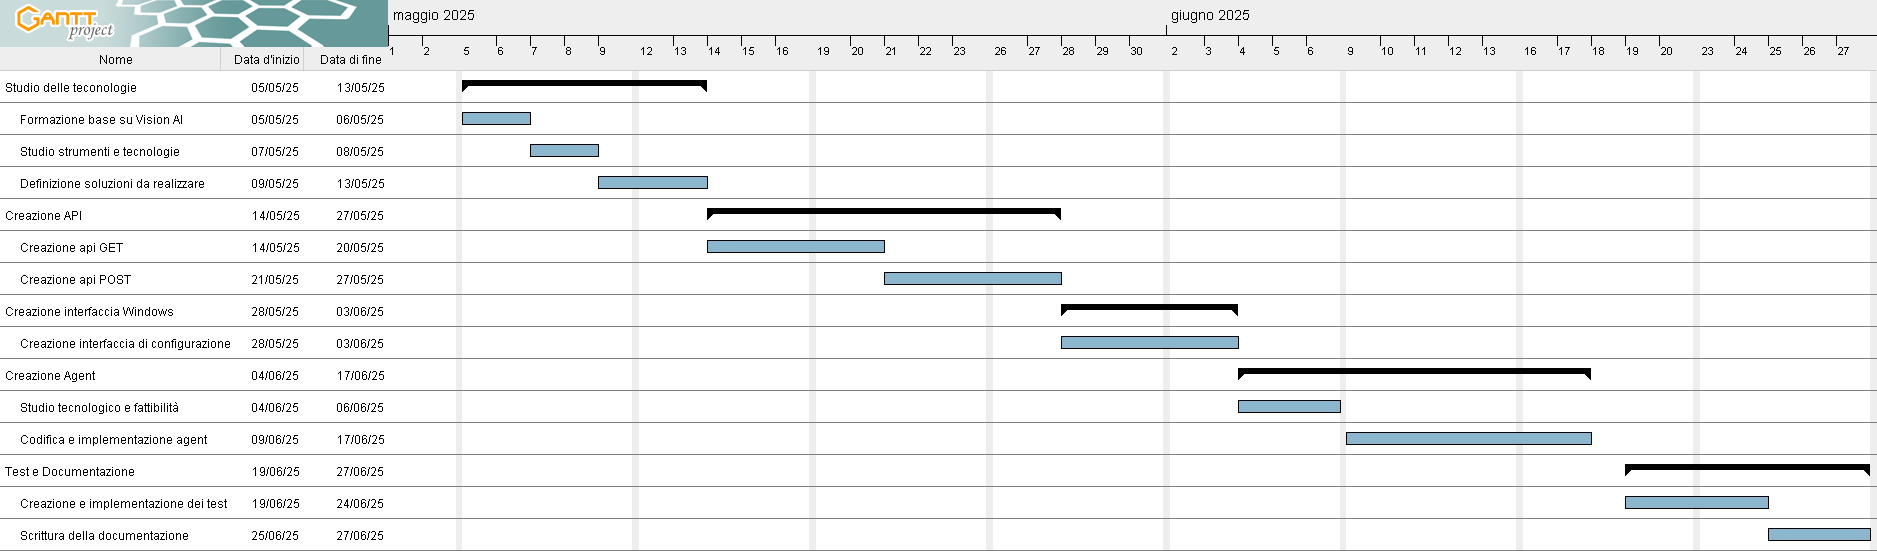
\includegraphics[width=\textwidth]{thesis/files/img/gaant.png}
    \caption{Pianificazione temporale dello \textit{stage}}
    \label{fig:pianificazione-stage}
\end{figure}

La struttura del lavoro all'interno del periodo di \textit{stage}, che è determinato da un monte ore limitato, è stata definita in collaborazione con il \textit{tutor} aziendale, suddividendo il tempo totale in sotto-periodi come illustrato nell'immagine \ref{fig:pianificazione-stage}. Questa divisione è avvenuta prima dell'inizio del tirocinio e presentata nel piano di lavoro.
Lo \textit{stage} è stato diviso in queste sezioni:
\begin{itemize}
    \item \textbf{Studio degli applicativi e del \textit{database}} (una settimana), l'obiettivo di questo periodo era l'apprendimento delle tecnologie e l'analisi del codice già presente, inoltre una prima formazione sulla struttura del \textit{database}.
    \item \textbf{Nuove \mygls{API}} (due settimane), in questo periodo è stata pianificata la creazione delle nuove \mygls{API} e perfezionare quelle già esistenti.
    \item \textbf{Interfaccia di configurazione} (una settimana), il periodo indicato allo sviluppo dell'interfaccia di connessione a VisionAI, creando un \textit{form} per la connessione al \textit{database} e alla \textit{chat}.
    \item \textbf{\textit{Agent}} (due settimane), l'obiettivo di questo periodo è la progettazione e lo sviluppo dell'\textit{agent} per la pianificazione automatica degli interventi.
    \item \textbf{\textit{Test} e documentazione} (una settimana e mezza), questo il periodo dedicato alla stesura della documentazione tecnica e allo svolgimento dei \textit{test}.
\end{itemize}

\textbf{Vincoli tecnologici generali}\\
L'azienda non ha imposto vincoli predefiniti a livello di tecnologie per la comunicazione e la documentazione, ma inserendosi in un contesto lavorativo già avviato comporta l'adozione di strumenti e metodologie già in uso.
% COMUNICAZIONE
\begin{figure}[H]
\centering
\begin{tikzpicture}[node distance=1cm and 2cm, every node/.style={font=\sffamily}, align=center]

  \node[draw, fill=white, minimum width=5.5cm, minimum height=3cm] (comunicazioni) at (0,0) {
    \textbf{Comunicazioni} \\[0.5em]
    \includegraphics[width=1cm]{thesis/files/img/Microsoft_Office_Outlook_(2018–present).svg.png} \\[-0.2em]
    Outlook \\[1em]
    \includegraphics[width=1cm]{thesis/files/img/Microsoft_Office_teams_(2018–present).svg.png} \\[-0.2em]
    Teams
  };

  \node[draw, fill=white, minimum width=5.5cm, minimum height=3cm, right=of comunicazioni] (doc) {
    \textbf{Documentazione} \\[0.5em]
    
\includegraphics[width=1cm]{thesis/files/img/word.png} \\[-0.2em]
    Word \\[1em]
    
\includegraphics[width=1cm]{thesis/files/img/2023_Obsidian_logo.svg.png} \\[-0.2em]
    Obsidian
  };
\end{tikzpicture}
\caption{Tecnologie utilizzate per la comunicazione e la documentazione.}
\label{fig:doc_com}
\end{figure}
La figura \ref{fig:doc_com} mostra le tecnologie utilizzate per le comunicazioni: 
\begin{itemize}
    \item Outlook: strumento di comunicazione utilizzato per lo scambio di posta elettronica con il referente aziendale o membri dei \textit{team} di sviluppo, per la gestione degli appuntamenti in calendario e per la pianificazione di incontri e riunioni.
    \item Microsoft Teams: strumento utilizzato in occasione della riunione mensile per rendere possibile la partecipazione di elementi non presenti direttamente in sede e per svolgere incontri di informazione organizzati dal \textit{tutor} aziendale con persone esterne.
\end{itemize}
 Gli strumenti per la documentazione sono i seguenti: 
 \begin{itemize}
     \item Microsoft Word: utilizzato principalmente per consultare e integrare la documentazione fornitaci dal \textit{tutor} aziendale e per integrare la seguente documentazione con i risultati dei \textit{test} svolti sul prodotto sviluppato.
     \item Obsidian: strumento utilizzato per redigere la documentazione tecnica in modo semplice e leggibile, utilizzato per organizzare appunti, annotazioni e idee durante il periodo di \textit{stage} tramite \textit{markdown}.
 \end{itemize}

 
\section{Vincoli tecnologici e obiettivi aziendali}
Il progetto come ho descritto nella sotto-sezione \ref{subs:Presentazione-progetto} è stato diviso in due componenti differenti, ognuno dei quali ha presentato vincoli tecnologici e obiettivi aziendali distinti.

\subsection{Assistente VisionAI}
L'azienda, come già detto, non impone vincoli tecnologici fissi, lasciando piena libertà nella decisione di linguaggi, \textit{framework} e ambienti di sviluppo.
Le scelte a livello di tecnologie da utilizzare quindi sono prese in maniera autonoma dallo stagista principalmente in base a efficacia e familiarità.
Nel caso specifico del progetto VisionAI, tuttavia, esisteva già una base di codice preesistente, sviluppata in C\#, e gli obiettivi concordati prevedevano espressamente l'utilizzo di questo linguaggio. In aggiunta durante lo sviluppo del prototipo iniziale erano già state prese anche altre scelte, è quindi stato opportuno mantenere lo \textit{stack} tecnologico già in uso per coerenza, visualizzabile nelle figure \ref{img:sviluppo} e \ref{fig:TecAI}

\textbf{Ambienti di sviluppo}
% SVILUPPO 
\begin{figure}[H]
\centering
\begin{tikzpicture}[node distance=2cm and 1.5cm, every node/.style={font=\sffamily}, align=center]

  % Blocco Sviluppo
  \node[draw, fill=white, minimum width=5cm, minimum height=3.8cm] (sviluppo) {
    \textbf{Ambienti di sviluppo} \\[0.5em]
    
\includegraphics[width=1cm]{thesis/files/img/vs.png} \\[-0.2em]
    Visual Studio \\[1em]
    
\includegraphics[width=1cm]{thesis/files/img/vscode.png} \\[-0.2em]
    Visual Studio Code \\[1em]
    
\includegraphics[width=1cm]{thesis/files/img/ssms.png} \\[-0.2em]
    SSMS
  };

\end{tikzpicture}
\caption{Ambienti di sviluppo per il modulo VisionAI.}
\label{img:sviluppo}
\end{figure}

\begin{itemize}
    \item Visual Studio: strumento utilizzato per la scrittura e il mantenimento del codice delle \mygls{API} tramite il supporto nativo al \textit{framework} .NET. scelto per i numerosi strumenti che fornisce a supporto dello sviluppo come strumenti di \textit{debug} e la gestione dei pacchetti.
    \item Visual Studio Code: utilizzato anche questo per lo sviluppo delle \mygls{API}, scelto principalmente per la familiarità con l'ambiente, per rendere più efficiente la scrittura del codice in determinati momenti.
    \item SQL Server Management Studio (SSMS): utilizzato per eseguire interrogazioni al \textit{database} relazione, supporta la scrittura di più \textit{query} in contemporanea e utilizzato per svolgere operazioni nel \textit{database} a supporto dello sviluppo.
\end{itemize}

\textbf{\textit{Framework} e \textit{software}}
\begin{figure}[H]
\centering
\begin{tikzpicture}[node distance=2cm and 2cm, every node/.style={font=\sffamily}, align=center]

  \node[draw, fill=white, minimum width=5.5cm, minimum height=4cm] (testing) at (0,0) {
    \textbf{\textit{Testing}} \\[0.5em]
    
\includegraphics[width=1cm]{thesis/files/img/swagger.png} \\[-0.2em]
    Swagger \\[1em]
    
\includegraphics[width=1cm]{thesis/files/img/postman.png} \\[-0.2em]
    Postman \\ [1em]
    
\includegraphics[width=1cm]{thesis/files/img/images.jpeg} \\[-0.2em]
    Ngrok 
  };

  \node[draw, fill=white, minimum width=5.5cm, minimum height=4cm, left=of testing] (API) {
    \textbf{Sviluppo \textit{API} e \textit{form}} \\[0.5em]
    
\includegraphics[width=1cm]{thesis/files/img/aspcore.png} \\[-0.2em]
    ASP.NET Core \\[1em]
    
\includegraphics[width=1cm]{thesis/files/img/entity_image.png} \\[-0.2em]
    Entity Framework \\[1em]
    
\includegraphics[width=1cm]{thesis/files/img/odata.png} \\[-0.2em]
    OData
  };

\end{tikzpicture}
\caption{Tecnologie utilizzate per il modulo VisionAI.}
\label{fig:TecAI}
\end{figure}
\begin{itemize}
    \item ASP.NET Core: \textit{framework} utilizzato per la scrittura delle \mygls{API} \mygls{REST}ful, permesso di sviluppare \mygls{endpoint}(url a cui un client può inviare richieste per eseguire operazioni sui dati) e mantenere alte le prestazioni
    \item Entity Framework Core: strumento \mygls{ORM}, tecnica che consente di interagire con \textit{database} in linguaggio di programmazione anzi che utilizzare \textit{query}, utilizzato per l'accesso ai dati.
    \item OData: Utilizzato per integrare funzionalità all'interno della \mygls{API} direttamente via URL, permettendo all'intelligenza artificiale di formulare \textit{query} con filtri direttamente all'interno dell'URL della chiamata
\end{itemize}

In merito alle tecnologie a supporto della fase di \textit{testing} delle \mygls{API} sono state:
\begin{itemize}
    \item Swagger: utilizzato per la generazione automatica della documentazione delle \mygls{API}, tramite la sua interfaccia inoltre è possibile esplorare le chiamate ed effettuare \textit{test} facilitando il \textit{debug}.
    \item Postman: tecnologia utilizzata per effettuare \textit{test} mirati, impiegato principalmente per \textit{testare} la funzionalità delle \mygls{API} POST.
    \item Ngrok: utilizzato per esporre in modo temporaneo il \textit{backend} e le \mygls{API} alla rete esterna, questo strumento ha permesso di \textit{testare} le chiamate all'interno della \textit{chat} senza dover pubblicare il servizio su un \textit{server} remoto.
\end{itemize}


\textbf{Obiettivi aziendali} \\
La tabella \ref{tab:obiettivi-aziendali} contiene gli obiettivi concordati con il \textit{tutor} aziendale previsti per la sezione corrente.
Gli obiettivi sono categorizzati in obbligatori, lettera O, desiderabili, lettera D, e facoltativi, lettera F.
\begin{table}[H]
\centering
\begin{tabular}{|c|p{11cm}|}
\hline
\textbf{Codice} & \textbf{Descrizione} \\
\hline
O01 & Sviluppo interfacce Visual Studio con librerie DevExpress \\
\hline
O02 & Sviluppo delle \mygls{API} di \textit{back-end} in linguaggio C\# \\
\hline
D01 & Creazione in autonomia della documentazione e del piano di \textit{test}  \\
\hline
\end{tabular}
\caption{Tabella obiettivi aziendali sezione VisionAI}
\label{tab:obiettivi-aziendali}
\end{table}


\subsection{Modulo di pianificazione interventi }
La sezione del progetto incentrata allo sviluppo dell'\textit{agent} per la pianificazione automatica degli interventi nel contesto di VisionAssistance è stato iniziato da zero, quindi ha concesso una libertà assoluta dal punto di vista tecnologico, la figura \ref{img:sviluppoa} mostra le scelte relative agli ambienti di sviluppo mentre la figura \ref{fig:Ag} mostra le scelte relative ai linguaggi e strumenti \textit{software} prese per questo modulo.

\textbf{Ambienti di sviluppo}
% SVILUPPO 
\begin{figure}[H]
\centering
\begin{tikzpicture}[node distance=2cm and 1.5cm, every node/.style={font=\sffamily}, align=center]

  % Blocco Sviluppo
  \node[draw, fill=white, minimum width=5cm, minimum height=3.8cm] (sviluppo) {
    \textbf{Ambienti di sviluppo} \\[0.5em]
    
\includegraphics[width=1cm]{thesis/files/img/vscode.png} \\[-0.2em]
    VS Code \\[1em]
    
\includegraphics[width=1cm]{thesis/files/img/ssms.png} \\[-0.2em]
    SSMS
  };

\end{tikzpicture}
\caption{Ambienti di sviluppo  per il modulo assegnazione interventi.}
\label{img:sviluppoa}
\end{figure}

\begin{itemize}
    \item Visual Studio Code: ambiente scelto per la scrittura del codice python, utilizzato per la familiarità con l'ambiente di sviluppo e la disponibilità di estensioni utili.
    \item SQL Server Management Studio (SSMS): impiegato per eseguire interrogazioni e operazioni sul \textit{database} aziendale, utile per la visualizzazione dei dati e verificare l'integrità dei dati utilizzati.

\end{itemize}

\textbf{Linguaggi e strumenti \textit{software}}

%\textit{agent}
\begin{figure}[H]
\centering
\begin{tikzpicture}[node distance=1cm and 2cm, every node/.style={font=\sffamily}, align=center]

  \node[draw, fill=white, minimum width=6cm, minimum height=3.5cm] (agent) at (0,0) {

    \textbf{Tecnologie \textit{software}} \\[0.5em]
    
\includegraphics[width=1cm]{thesis/files/img/python.png} \\[-0.2em]
    Python \\[1em]
    
\includegraphics[width=1cm]{thesis/files/img/sqlA.png} \\[-0.2em]
    SQLAlchemy \\[1em]
    
\includegraphics[width=1cm]{thesis/files/img/orLogo.png} \\[-0.2em]
    OR-Tools
  };

\end{tikzpicture}
\caption{Tecnologie utilizzate per il modulo di pianificazione interventi.}
\label{fig:Ag}
\end{figure}
\begin{itemize}
    \item Python: Linguaggio di programmazione principale utilizzato per lo sviluppo di questo progetto, scelto per la sintassi semplice, la familiarità e per la compatibilità con OR-Tools.
    \item SQLAlchemy: libreria \mygls{ORM} utilizzata per gestire l'accesso ai dati. Infatti, permette di scrivere \textit{query} in linguaggio SQL direttamente all'interno del codice per facilitare l'accesso ai dati.
    \item Google OR-Tools: \textit{solver} per la programmazione vincolata, è stato utilizzato per risolvere il problema dell'assegnazione ottimale degli interventi.
\end{itemize}

\textbf{Obiettivi aziendali}\\
La tabella \ref{tab:obiettivi-aziendali-interventi} contiene gli obiettivi concordati con il \textit{tutor} aziendale previsti per la sezione del progetto di stage in questione.
Il codice identificativo è il medesimo della sezione precedente.
\begin{table}[H]
\centering
\begin{tabular}{|c|p{11cm}|}
\hline
\textbf{Codice} & \textbf{Descrizione} \\
F01 &  Creazione di un \textit{agent} per la pianificazione degli interventi in VisionAssistance \\
\hline
\end{tabular}
\caption{Tabella obiettivi aziendali per sezione pianificazione interventi}
\label{tab:obiettivi-aziendali-interventi}
\end{table}







\section{Obiettivi personali}
La tabella \ref{tab:obiettivi-personali} mostra invece gli obiettivi personali stipulati prima dell'inizio dello \textit{stage}, la notazione degli obiettivi è la stessa delle tabelle precedenti.

\begin{table}[H]
\centering
\begin{tabular}{|c|p{11cm}|}
\hline
\textbf{Codice} & \textbf{Descrizione} \\
\hline
O01 & Imparare nuove tecnologie e \textit{framework} legati all'ambiente .NET e al linguaggio C\# \\
\hline
O02 & Collaborare attivamente con il \textit{team}, mantenendo una comunicazione efficace e continua \\
\hline
O03 & Svolgere le attività nel rispetto delle scadenze concordate. \\
\hline
D01 & Ampliare il mio bagaglio tecnico e di \textit{soft-skill} in un contesto strutturato \\
\hline
\end{tabular}
\caption{Obiettivi personali dello \textit{stage}.}
\label{tab:obiettivi-personali}
\end{table}




\newpage